%%%%%%%%%%%%%%%%%%%%%%%%%%%%%%%%%%%%%%%%%%%%%%%%%%%%%%%%%%%%%%%%%%
\section{Inteligencia Artificial}
\label{sec:ml}

La inteligencia artificial (\gls{ia}) se constituye como la disciplina de diseño y creación de sistemas de software o hardware de imitación de la inteligencia humana para la realización de tareas. Generalmente, estos sistemas obtienen la capacidad de aprendizaje, razonamiento, planificación y toma de decisiones a partir del entrenamiento basado en grandes cantidades de información. En otros términos, adquieren e interpretan datos del entorno o de un contexto específico y, teniendo en cuenta un objetivo determinado, procesan la información contenida para decidir la siguiente acción a realizar. Adicionalmente, son capaces de adaptar su comportamiento ante el análisis o detección de cambios en el entorno. \cite{iagov} \cite{iaazure}

\vspace{3mm}

La \gls{ia} se determina como una de las tecnologías más revolucionarias y transformadoras de la actualidad y del futuro cercano por su potencial de aplicación en numerosos ámbitos. No obstante, el origen del término se remonta al año 1956, cuando el científico John McCarthy introdujo la idea de crear máquinas inteligentes tomando como base las teorías de computación de los matemáticos Norbert Wiener y John von Neumann en los años 40.~\cite{iagov}

\vspace{3mm}

En la última década, el impulso de la \gls{ia} y los grandes avances que se han producido en este campo vienen dados principalmente, por el aumento de las capacidades de los equipos informáticos y el acceso a grandes cantidades de recursos computacionales en las herramientas especializadas e infraestructuras de nube. En otros términos, se posibilita un almacenamiento masivo de datos y, en consecuencia, mejoras significativas en el desarrollo de algoritmos y técnicas, que cada vez se vuelven más complejas y precisas. 

\vspace{3mm}

Entrando en estas técnicas, se establecen dos divisiones dentro del campo de la \gls{ia} en función de la naturaleza del aprendizaje: el automático (\acrfull{ml}) y el profundo (\acrfull{dl}). En las siguientes Secciones (ver Secciones \ref{sec:ml} y \ref{sec:dl}) se expondrán las características que presentan cada una de estas ramas, además de entrar en profundidad en el funcionamiento de los modelos que se emplearán en el desarrollo de este \gls{tfm}.

\subsection{Machine Learning (\acrshort{ml})}
\label{sec:ml}

La rama de aprendizaje automático (\acrfull{ml}) se enfoca en el desarrollo de modelos que sean capaces de aprender y tomar decisiones en base a la introducción de datos. Durante el proceso se realizan observaciones a la información existente y, en función de la técnica a emplear, se aplican algoritmos estadísticos para identificar patrones en los datos. Por lo tanto, mediante un entrenamiento progresivo en el tiempo, un modelo de \gls{ml} puede llegar a realizar predicciones sobre datos futuros sin la intervención humana y con una alta precisión. Como se representa en la Figura \ref{fig:ml}, las técnicas de \gls{ml} pueden pertenecer a tres categorías diferentes en función del enfoque de la información y de los objetivos que se pretenden conseguir con su aplicación: \cite{mlcat} \cite{iageeks} \cite{mltlf}

\begin{itemize}
    \item Aprendizaje no supervisado: Se parte de datos sin etiquetar para el entrenamiento de los modelos. Es decir, se parte del conocimiento de unos datos de entrada, pero no de la salida, por lo que el objetivo de los modelos no supervisados se basa en explorar posibles patrones en los datos mediante clustering.
    \item Aprendizaje supervisado: Se manejan conjuntos de datos con un conocimiento de las posibles salidas, las cuales se proporcionan en forma de etiquetas o de valores numéricos. Las técnicas de aprendizaje supervisado buscan un función óptima que consiga, dadas unas determinadas variables o características de entrada, predecir la salida con cierta precisión y son aplicables a dos tipos de problemas: de regresión, si a partir de las variables de entrada se desea predecir un valor numérico continuo a la salida, o de clasificación, si se predefinen diferentes clases y se asignan las variables de entrada a una de ellas. 
    \item Aprendizaje por refuerzo: Las técnicas englobadas en este tipo aprenden por prueba y error, por lo que su entrenamiento a lo largo del tiempo y la experiencia permiten optimizar los resultados sin la necesidad de disponer de un gran volumen de datos.
\end{itemize}

\begin{figure}[h!]
    \centering
    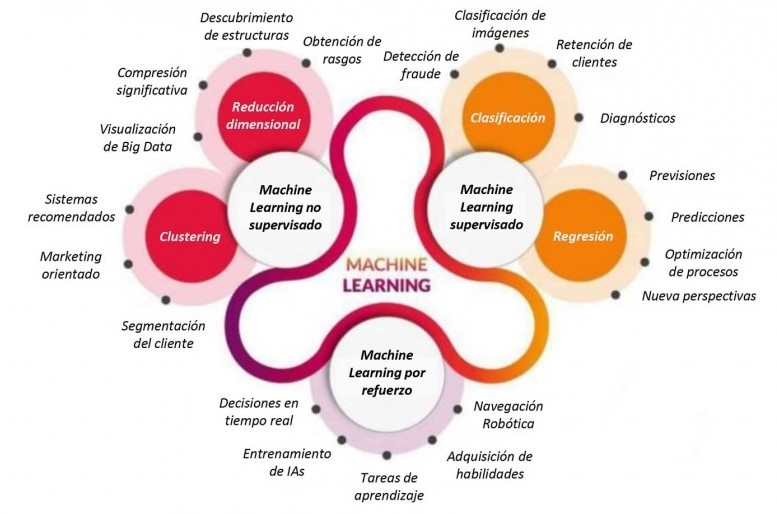
\includegraphics[width=1\textwidth]{img/teoria/ml.jpeg}
    \caption{Categorías de \acrshort{ml} \cite{metal}}
    \label{fig:ml}
\end{figure}

\vspace{3mm}

Una vez expuestas las diferentes categorías donde se engloban las técnicas de \gls{ml}, es preciso indicar que se va a centrar el estudio en el aprendizaje supervisado y, en particular, en la resolución de problemas de clasificación binaria. El motivo principal viene dado porque el objetivo que se persigue con la realización de este \gls{tfm} se basa en el desarrollo de modelos que permitan detectar y predecir posibles errores que se pueden producir en una \gls{sg} durante el proceso de distribución energética. 

\vspace{3mm}

Como se detallará más adelante en la Sección \ref{sec:cambiosden2ne}, se creará un conjunto de datos etiquetados en función de la existencia de error o no para entrenar los modelos. Teniendo en cuenta esto, a continuación, se incluyen dos Secciones (ver Secciones \ref{sec:mlsvm} y \ref{sec:mlrf}) para presentar el funcionamiento de las dos técnicas de \gls{ml} que se desarrollarán posteriormente.

\subsubsection{Random Forest (\acrshort{rf})}
\label{sec:mlrf}







\subsubsection{Support Vector Machines (\acrshort{svm})}
\label{sec:mlsvm}

El algoritmo de Máquinas de Vector Soporte (del inglés \gls{svm}) es una técnica que se emplea tanto en problemas de regresión como de clasificación. Se basa en el concepto del \textit{Maximal Margin Classifier} o \textit{Hard Margin Classifier}, puesto que tiene el fin principal de encontrar el hiperplano óptimo que consiga una máxima separación entre dos clases diferentes dentro de un espacio de características. Esta separación se define como margen y se mide como la distancia perpendicular que existe desde el hiperplano hacia los vectores de soporte, que son las muestras más cercanas a la frontera de separación de clases. En la Figura \ref{fig:svm} se representa el cálculo del mejor hiperplano entre dos clases de datos. \cite{svmmedium2} \cite{svmciencia}

\vspace{3mm}

\begin{figure}[h!]
    \centering
    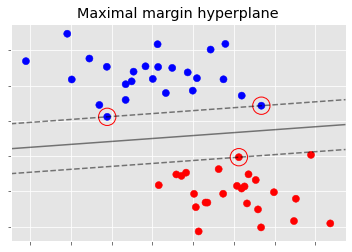
\includegraphics[width=0.65\textwidth]{img/teoria/svm.png}
    \caption{Cuantificación del hiperplano óptimo entre dos clases en el \acrshort{svm} \cite{svmmedium2}}
    \label{fig:svm}
\end{figure}

\vspace{3mm}

Por ello, se puede expresar que los vectores de soporte son los puntos más críticos del plano para asignar una de las clases predefinidas a los nuevos vectores de datos a la entrada. Este proceso de clasificación viene dado por la siguiente expresión: \cite{svmmedium} 

\[ y_i(\mathbf{w} \cdot \mathbf{x_i} + b) \geq M\]

    Donde:
\begin{itemize}
    \renewcommand{\labelitemi}{}
    \item \(y_i\) es la etiqueta de la clase. 
    \item \(x_i\) es el vector de características.
    \item \(w\) es el vector de pesos o coeficientes del hiperplano.
    \item \(b\) es el sesgo ajustado en el modelo.
    \item \(M\) es el ancho definido para el margen.
\end{itemize}

\vspace{3mm}

No obstante, en la práctica es complicado determinar un hiperplano si no se trata de un problema ideal y basado en datos linearmente separables. Generalmente, en los casos reales si se intenta forzar un máximo margen, se pueden llegar a producir problemas de sobreentrenamiento, ya que nuevos datos pueden suponer grandes variaciones en el hiperplano. En la Figura \ref{fig:svmerror} se representa la opción alternativa que se lleva a cabo en la mayoría de casos, basada en obtener un margen máximo, permitiendo cierto grado de error (\textit{Soft Margin Classifier}). \cite{matlab} \cite{svmciencia}

\vspace{3mm}

\begin{figure}[h!]
    \centering
    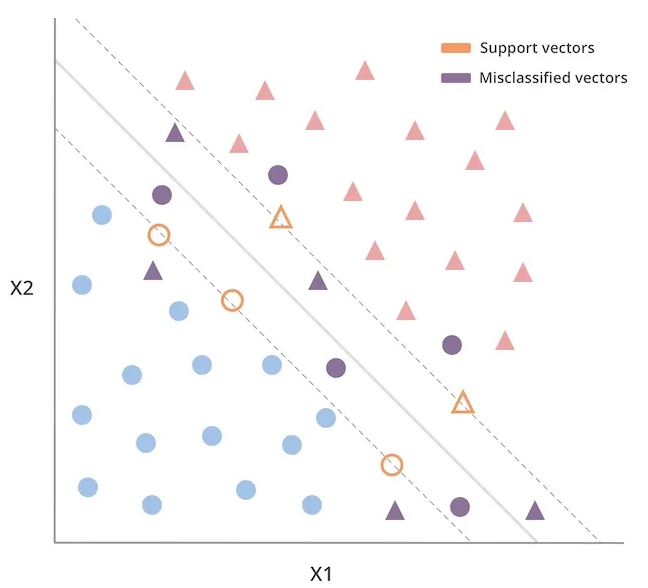
\includegraphics[width=0.55\textwidth]{img/teoria/svm2.png}
    \caption{Representación de vectores clasificados erróneamente dentro de los márgenes establecidos en el \acrshort{svm} \cite{svmmedium}}
    \label{fig:svmerror}
\end{figure}

\vspace{3mm}

Esto tiene como consecuencia que existan una serie de vectores clasificados de forma errónea en el plano. En este proceso se introduce el concepto de variables de holgura (\textit{slack variables}) a partir de la siguiente expresión:

\[ \xi_i = \max(0, 1 - y_i (\mathbf{w} \cdot \mathbf{x}_i + b))\]

Estas variables determinan si un vector está correctamente clasificado o si se encuentra en una zona errónea del margen o del hiperplano, respectivamente. En el caso de posición incorrecta, el valor de la variable define la distancia al margen o el error cometido:

\[\begin{array}{ll}
    \xi_i = 0 & \text{si } 1 - y_i (\mathbf{w} \cdot \mathbf{x}_i + b) \leq 0 \\
    0 \text{<} \xi_i \text{<} 1 & \text{si } 0 < 1 - y_i (\mathbf{w} \cdot \mathbf{x}_i + b) \leq 1 \\
    \xi_i \text{>} 1 & \text{si } 1 - y_i (\mathbf{w} \cdot \mathbf{x}_i + b) > 1 \\
\end{array}\]

\vspace{3mm}

El sumatorio de todas las variables de holgura que existen en el plano vienen incluidas en el objetivo de la función de pérdida del modelo para que el error de clasificación sea mínimo, a la vez que el margen es máximo. Como es preciso encontrar un cierto equilibrio entre ambos, el \gls{svm} se determina como una técnica de optimización convexa que se fundamenta en el hiperparámetro \textit{C}. En la Figura \ref{fig:parametroc} se representa de forma gráfica cómo su valor establece el control de forma inversamente proporcional de la cantidad de muestras clasificadas erróneamente, por lo que se define como el parámetro de regularización del modelo. Es decir, cuanto más alto sea su valor, menores violaciones del margen y del hiperplano serán permitidas y más se enfocará el modelo en un \textit{Maximal Margin Classifier}.~\cite{svmciencia}

\vspace{3mm}

\begin{figure}[h!]
    \centering
    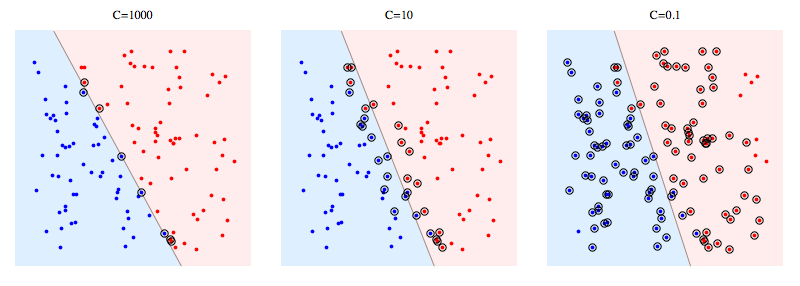
\includegraphics[width=1\textwidth]{img/teoria/parametroc.png}
    \caption{Configuración del parámetro de regularización \textit{C} \cite{velocity}}
    \label{fig:parametroc}
\end{figure}

\vspace{3mm}

Para enfrentar problemas con datos no linearmente separables, además de permitir cierto grado de error, como se ha expuesto anteriormente, es imprescindible incrementar las dimensiones del espacio original de características. En este caso se introduce el concepto de kernel como función para obtener un nuevo espacio dimensional diferente al original donde exista una mayor probabilidad de que los datos sean linearmente separables. La aplicación de los diferentes tipos de kernels se caracterizan por las siguientes expresiones:~\cite{svmciencia}~\cite{velocity}

\[\begin{array}{ll}
    \text{Kernel lineal: } & K(\mathbf{x}_i, \mathbf{x}_j) = \mathbf{x}_i \cdot \mathbf{x}_j\\
    \text{Kernel polinómico: } & K(\mathbf{x}_i, \mathbf{x}_j) = (\gamma \mathbf{x}_i \cdot \mathbf{x}_j + r)^d\\
    \text{Kernel radial o gaussiano: } & K(\mathbf{x}_i, \mathbf{x}_j) = \exp \left( -\gamma \| \mathbf{x}_i - \mathbf{x}_j \|^2 \right)\\
    \text{Kernel sigmoid: } & K(\mathbf{x}_i, \mathbf{x}_j) = \tanh(\gamma \mathbf{x}_i \cdot \mathbf{x}_j + r)\\
\end{array}\]

\vspace{3mm}

De forma adicional, en la Figura \ref{fig:rbf} se representa cómo se produce la transformación dimensional de las características para el caso del kernel gaussiano o \gls{rbf}.

\vspace{3mm}

\begin{figure}[h!]
    \centering
    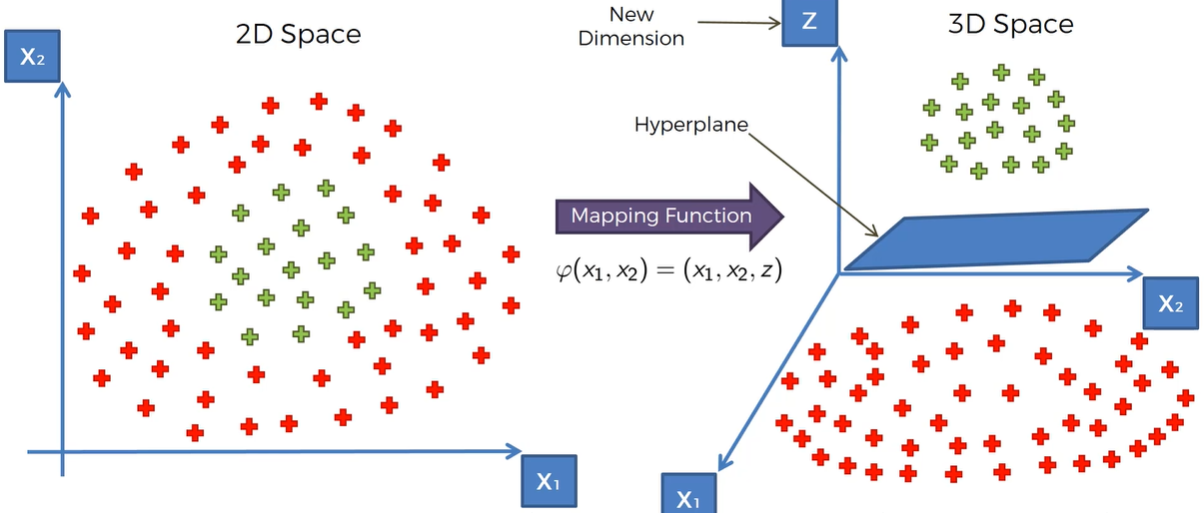
\includegraphics[width=1\textwidth]{img/teoria/rbf.png}
    \caption{Aplicación del kernel \acrshort{rbf} \cite{rbf}}
    \label{fig:rbf}
\end{figure}

\subsection{Deep Learning (\acrshort{dl})}
\label{sec:dl}

El campo del aprendizaje profundo (\acrfull{dl}) se enfoca principalmente en la creación de redes neuronales que imiten el comportamiento y la estructura lógica que tiene el cerebro humano para buscar patrones en los datos. A diferencia de las técnicas de \gls{ml}, el \gls{dl} se vuelve más eficiente en el análisis de grandes volúmenes de datos, puesto que el \gls{ml} presenta ciertas limitaciones en este aspecto. \cite{metal} 

\vspace{3mm}

De la misma forma, el \gls{dl} presenta un mejor funcionamiento en la identificación de patrones cuando se manejan características complejas, aportando resultados con una mayor precisión que el \gls{ml}. Es por ello que las técnicas de \gls{dl} cobran una gran importancia en entornos donde los datos no son estructurados, como se produce en el caso de las imágenes, texto y audio. En este caso se pueden introducir en aplicaciones de reconocimiento de voz, procesado de lenguaje natural (\gls{nlp}) o visión artificial para la detección de objetos y clasificación de imágenes. \cite{iageeks}

\vspace{3mm}

Por otro lado, a nivel estructural las diferencias entre las técnicas de \gls{ml} y las de \gls{dl} radican principalmente en el tratamiento de las características o variables de los datos. En el caso de emplear \gls{ml}, si se manejan conjuntos con un gran número de características, sería necesario introducir un paso previo de diseño y selección de las más relevantes. Esto, como se puede apreciar en la Figura \ref{fig:features}, no ocurre en el desarrollo de un modelo de \gls{dl}, ya que el tratamiento se produce internamente dentro de la red reuronal. \cite{valohai}

\vspace{3mm}

\begin{figure}[h!]
    \centering
    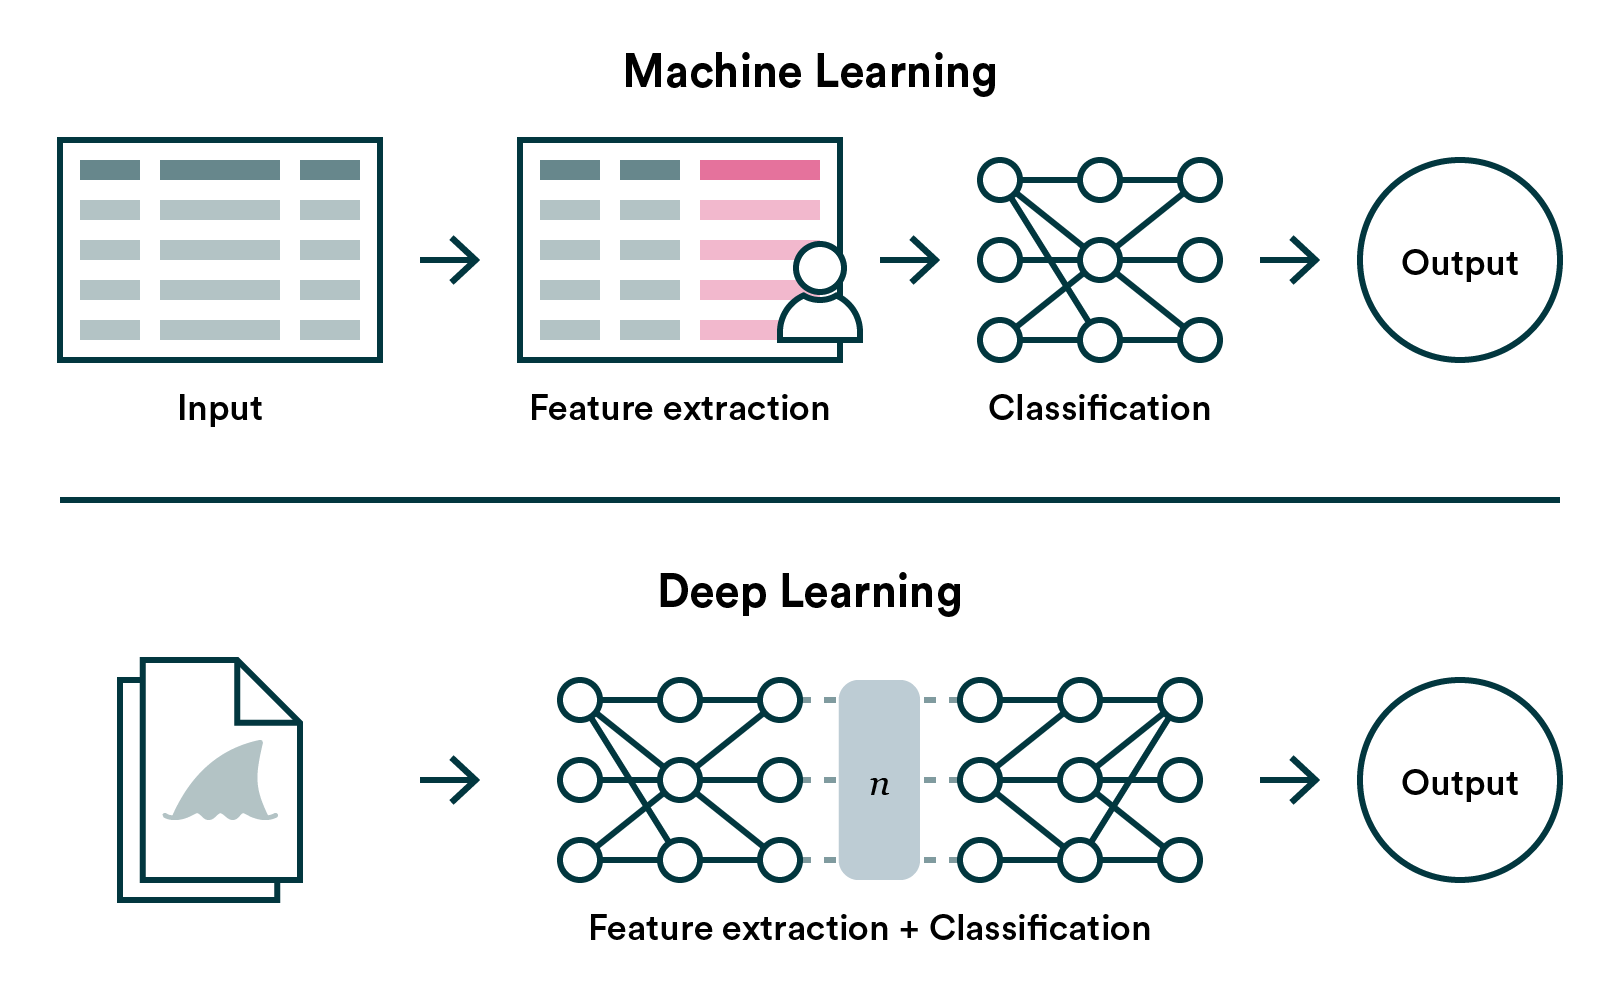
\includegraphics[width=0.85\textwidth]{img/teoria/mlvsdl.png}
    \caption{Diferencias estructurales entre el \acrshort{ml} y el \acrshort{dl} \cite{valohai}}
    \label{fig:features}
\end{figure}

\vspace{3mm}

Una vez definida la rama de aprendizaje profundo, además de presentar las diferencias que presenta respecto a la de aprendizaje automático, se introduce una Sección dedicada a la exposición del modelo de \gls{dl} que se desarrollará como motivo del objetivo de este \gls{tfm} (ver Sección \ref{sec:dlann}). 

\subsubsection{Red Neuronal Artificial (\acrshort{ann})}
\label{sec:dlann}

Las redes neuronales artificiales (\gls{ann})




% de procesamiento de información

% Se modelan múltiples capas de neuronas para procesar los datos de entrada y aprender a través de un proceso iterativo de ajuste de los pesos de las conexiones entre neuronas.

% Además, tiene la capacidad de identificar patrones y características más complejas en los datos, lo que puede llevar a mejores resultados en aplicaciones como el reconocimiento de voz, la visión por computadora y el procesamiento del lenguaje natural.




\vspace{3mm}

\begin{figure}[h!]
    \centering
    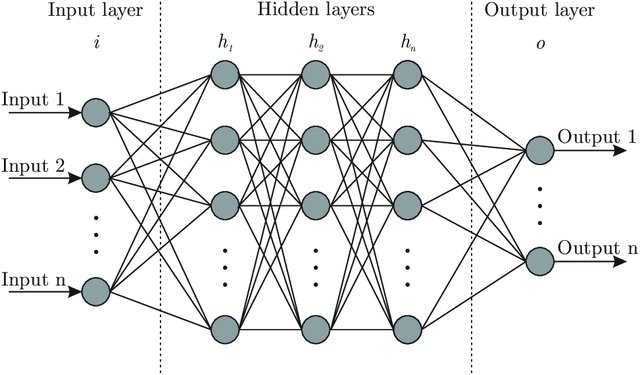
\includegraphics[width=0.8\textwidth]{img/teoria/ann.jpg}
    \caption{Arquitectura de una \acrshort{ann} \cite{ann}}
    \label{fig:features}
\end{figure}

\vspace{3mm}







%hablar sobre ml
%relacionar ml con sg
\cite{impact}


%aqui hablar de ml para eficiencia de consumo


%ver figura pag6 cite stab -> esquema acciones desarrollo







%cite stab (para que se usan los algoritmos)

% Los algoritmos de predicción se utilizan para estimar la oferta y la demanda.
% de la red (Wang et al., 2018). En Singh y Yassine (2018), el
% Se abordó el análisis de datos de medidores inteligentes y se propusieron tres principales
% Aplicaciones: análisis de carga, previsión de carga y gestión de carga. El
% Las técnicas clave para estas aplicaciones incluyen series temporales, agrupación de datos, reducción de dimensionalidad, clasificación de datos, detección de valores atípicos,
% matriz de bajo rango y aprendizaje en línea. En Kezunovic et al. (2013), un
% Se propuso un modelo de minería de datos inteligente que se puede utilizar para analizar,
% predecir y visualizar patrones de consumo de series temporales de energía. A
% La parte clave de este modelo fue el uso de "minería de patrones frecuentes"; frecuente
% Los patrones son conjuntos de elementos que aparecen en un conjunto de datos con una frecuencia igual.
% o más que un umbral especificado por el usuario. La minería de patrones frecuente es una
% Herramienta de minería de datos esencial para procesar y analizar big data.



